%%%%%%%%%%%%%%%%%%%%%%%%%%%%%%%%%%%%%%%%%%%%%%%%%%%%%%%%%%%%%%%%%%%%%%%%%%%%%%%%%%
\begin{frame}[fragile]\frametitle{}
\begin{center}
{\Large Ashtang अष्टांग }
\end{center}
\end{frame}

%%%%%%%%%%%%%%%%%%%%%%%%%%%%%%%%%%%%%%%%%%%%%%%%%%%%%%%%%%%
\begin{frame}[fragile]\frametitle{Patanjali}


	\begin{itemize}
	\item Patanjali was shastri of 3 shastras : Yog, Vyakaran, Ayurved
	\item He did tika/analysis of Panaini's vyakaran (``mahabhashya'')
	\end{itemize}


\end{frame}



%%%%%%%%%%%%%%%%%%%%%%%%%%%%%%%%%%%%%%%%%%%%%%%%%%%%%%%%%%%
\begin{frame}[fragile]\frametitle{Introduction}
``Yama Niyamasana Pranayama Pratyahara Dharanadhyana Samadhyoshta angani |''

यम-नियमासन-प्राणायाम-प्रत्याहार-धारणा-ध्यान-समाधयोऽष्टवङ्गानि ||

\end{frame}


%%%%%%%%%%%%%%%%%%%%%%%%%%%%%%%%%%%%%%%%%%%%%%%%%%%%%%%%%%%
\begin{frame}[fragile]\frametitle{8 Facets of Yog}

\begin{center}
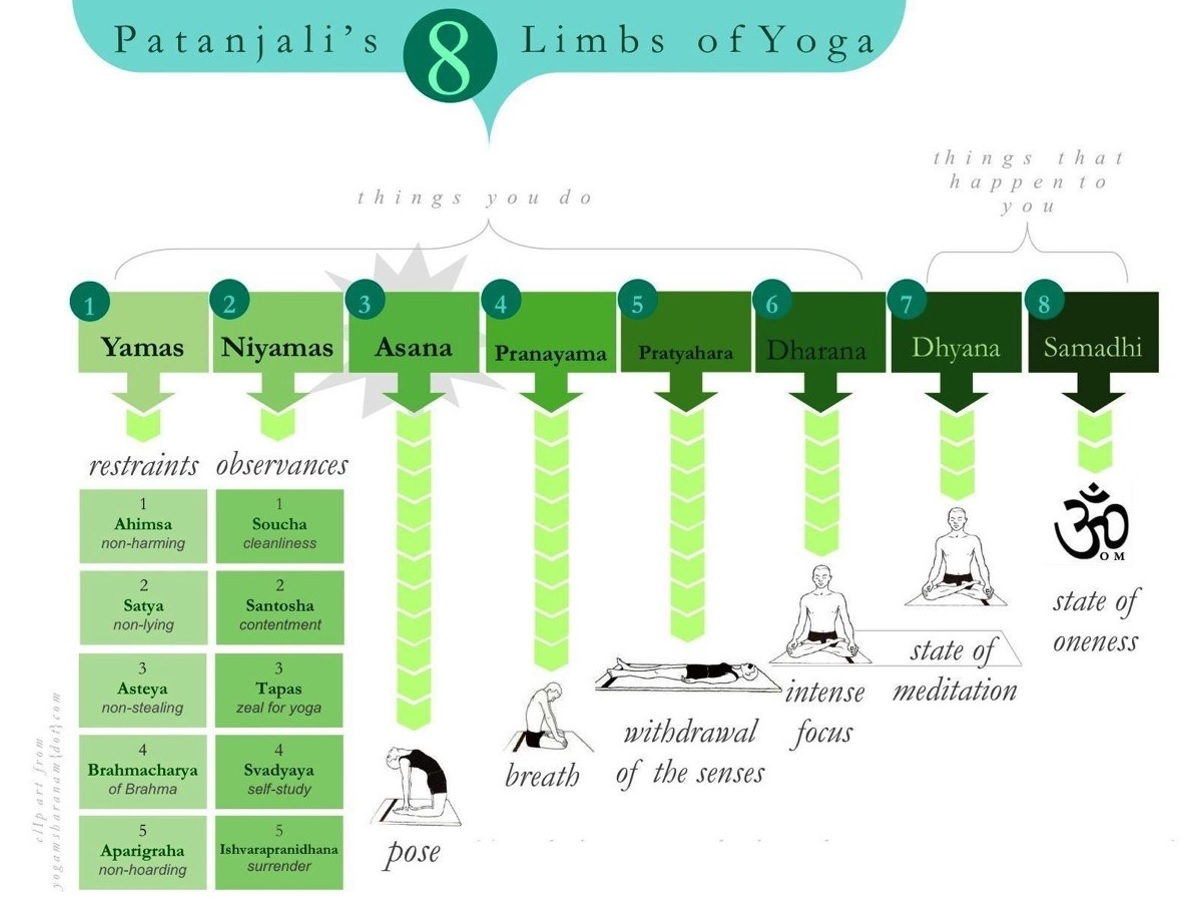
\includegraphics[width=\linewidth,keepaspectratio]{yog23}

\tiny{(Ref: Philosophy III - The Yoga SPace - Chandrika Gibson)}
\end{center}

\end{frame}

%%%%%%%%%%%%%%%%%%%%%%%%%%%%%%%%%%%%%%%%%%%%%%%%%%%%%%%%%%%
\begin{frame}[fragile]\frametitle{Yog : Transition from Body to Mind}

\begin{center}
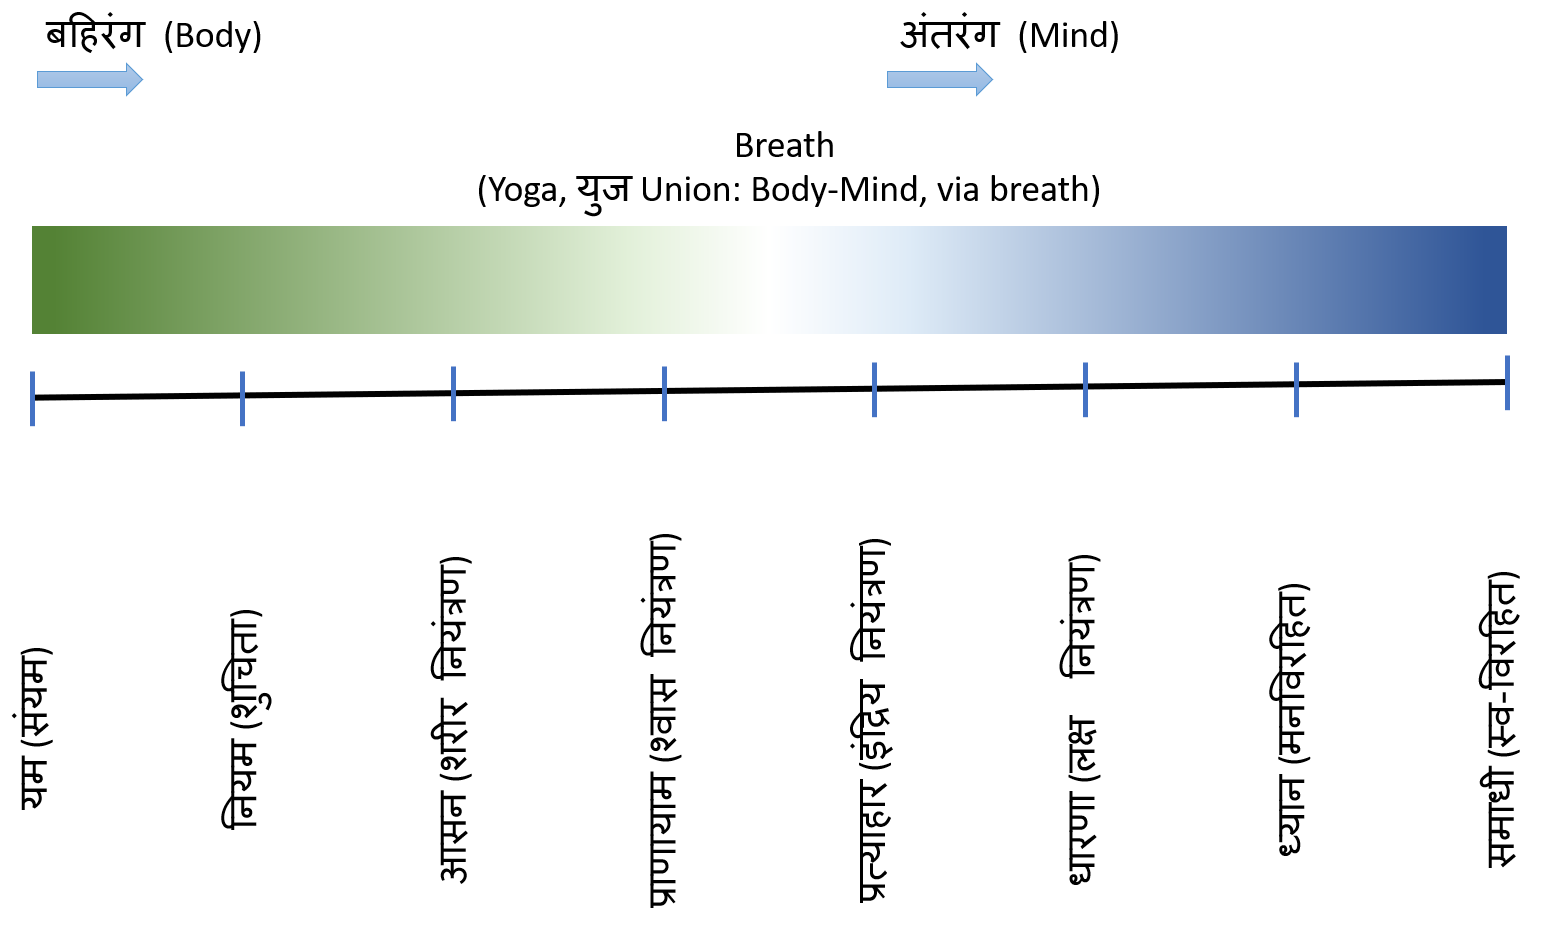
\includegraphics[width=\linewidth,keepaspectratio]{yogascale}

\end{center}

\end{frame}